
\section{Objetivo da equipe de transmissão de calor}
O objetivo do grupo de transmissão de calor, é determinar às temperaturas e as influências térmicas existentes no sistema, prioritariamente no que tange à esfera da câmara de combustão e suas derivadas. Assim, é de fundamental importância e incumbência do grupo, analisar os riscos da solução estabelecida, determinar diretrizes à outros grupos como o de estruturas e controle, e por fim definir os custos de materiais (bill of materials) e mão de obra utilizados na transmissão de calor.
\section{Metodologia}
Foi determinado quais atividades teriam maior importância durante o desenvolvimento do projeto como um todo e o tempo demandado para cada uma. Desta forma, foi produzido um cronograma com as datas das aulas de desenvolvimento do projeto e os três pontos de controle. Posteriormente, para a realização das pesquisas o grupo se subdividiu em sub-equipes de forma que fosse adquirido uma maior quantidade de material para um embasamento teórico mais profundo para o projeto a fim de que esse pudesse ser realizado em tempo hábil. Logo após a primeira etapa do projeto ser concluída, a equipe foi subdividida novamente nos seguintes grupos: conceito e documentação, simulações, tubulações e modelos matemáticos/físicos aplicáveis.\\
Uma determinação precisa do fluxo de calor é uma importante tarefa para o projeto e para o cálculo do desempenho de motores-foguete, dessa forma após os dados coletados e analisados há uma distribuição de informações entre os grupos restantes, com foco principal no grupo de estruturas onde os dados funcionam como pré-requisito. Com tais dados sobre o projeto, o fluxo de calor na câmara de combustão de motores-foguete com geometria cilíndrica serão calculados utilizando-se das equações newtonianas de temperatura e posteriormente será simulado por meio do programa ANSYS versão R18.1 e  R18.2 Academic. 
\section{Pontos de controle anteriores}
No primeiro ponto de controle, existiam duas possibilidades para a localidade do sensor na pré-câmara e pós-câmara. Dessa forma, após vários estudos mais aprofundados ficou definido que o sensor estará instalado na pós-câmara, isto é, entre o propelente sólido e a tubeira, sendo ele separado por um tubo cilíndrico à uma altura de $100mm$ do corpo principal da câmara.\\
Neste documento a parte de Transmissão de calor compõe os estudos na área de transmissão térmica do motor, do sensor e do líquido de arrefecimento. Destarte, as informações subsequentes determinam o estudo teórico e simulado do projeto.\\
Assim, utilizando os conhecimentos adquiridos pelas pesquisas realizadas, foram determinadas as equações que seriam utilizadas. Definiu-se então a equação da taxa de fluxo de calor (Equação ~\ref{eq1tc}) e a equação de propagação de calor em cilindros (ideal) no sentido radial (Equação ~\ref{eq2tc}), as quais o grupo se baseou para a formação sólida de uma solução.
\begin{equation}\label{eq1tc}
P_{cond}=\frac{\Delta Q}{\Delta t}=\frac{KA\Delta T}{L}
\end{equation}
\begin{equation}\label{eq2tc}
Q_{cond}=k_t.4.\pi.r_0.r_i.\frac{T_{S0}-T_{Si}}{r0-ri}
\end{equation}
As variáveis $K_t,r_0,r_i,T_{S0},T_{Si},r0,ri$ dizem respeito às dimensões da aproximação cilíndrica do adaptador como mostra a figura ~\ref{fig3tc} a seguir.
\begin{figure}[!htb]                  
	\centering                          
	
\includegraphics[scale=1]{figuras/Figura3tc.eps}
	\caption{Especificação das dimensões utilizadas}\label{fig3tc}               
\end{figure}
\section{Análise Teórica}
\subsection{Análise da câmara de combustão-Temperatura de parede}
A análise da câmara de combustão está relacionada à temperatura de parede, uma vez que o sistema de arrefecimento está apenas ligado a ela através do adaptador. De acordo com os dados disponíveis e com o conhecimento de que a câmara de combustão utilizada pela universidade é de tamanho laboratorial foi possível perceber que existe muita bibliografia nesse contexto, por isso a análise da temperatura de parede se baseou no gráfico apresentado na figura ~\ref{fig1tc} abaixo, na qual a temperatura sensível ao termopar é de 800ºC mas pela alta temperatura seu erro pode se estender em 20\%, o que é comprovado pela bibliografia que revela a temperatura na câmara exposta às mesmas condições.
\begin{figure}[!htb]                  
	\centering                          
	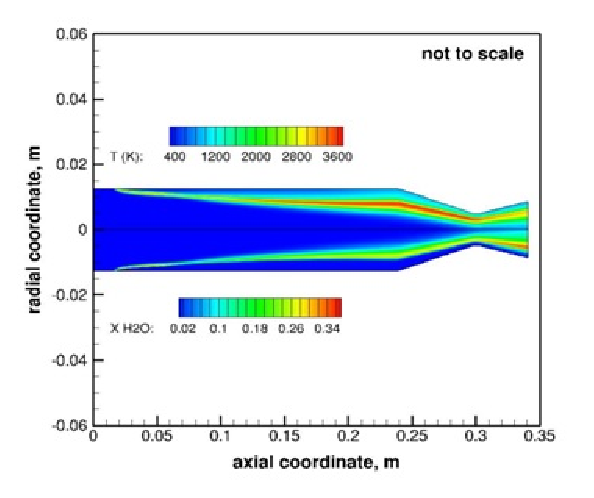
\includegraphics[scale=1]{figuras/Figura1tc.eps}
	\caption{Gráfico de temperatura}\label{fig1tc}               
\end{figure}
\newpage
\subsection{Análise do adaptador}
O adaptador (Figura ~\ref{fig2tc}) é a única conexão entre a câmara de combustão e o sensor de pressão, ele tem Ø = 19 mm, L = 100 mm e contém, uma parte hexagonal à 30 mm do início de mesmo tamanho do diâmetro e comprimento de 30 mm, um furo rosqueado com Ø = 11,5 mm seguido por um furo até o final do comprimento de Ø =3 mm e um apêndice com um pescoço de 2 mm e cabeça rosqueada de 8,5 mm, feito inteiramente do aço inoxidável AISI 304 L.\\
Com essas especificações, a temperatura se distribui na seção transversal, com área de$ 1,105 x10^{-3}m^2$, de acordo com condução e convecção, mas a distribuição por radiação foi desconsiderada por se tratar de um furo com área de $2,827 x 10^{(-5)}m^2$, cerca de 2,55\% da área da seção sólida, visto que, o furo não é preciso nem uniforme dificultando a propagação de calor.
\begin{figure}[!htb]                  
	\centering                          
	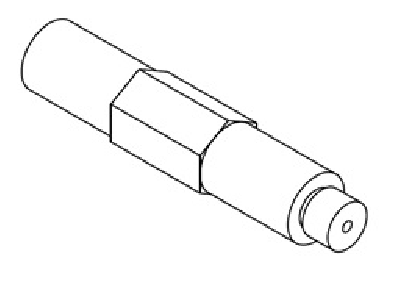
\includegraphics[scale=1]{figuras/Figura2tc.eps}
	\caption{Esquemático do adaptador} \label{fig2tc}              
\end{figure}
\subsection{Análise de temperatura no sensor}
O sensor é prioritariamente feito de aço e sua massa comparada à massa do cilindro adaptador, que tem massa de 0,867 Kg utilizando 7,85 g/cm3 como densidade do aço inox, e o sensor que pesa 18g, representando 2,07\% da massa do cilindro, podemos adotar então a temperatura do final do adaptador como a temperatura do sensor visto que sua massa é pequena comparada a temperatura do cilindro.
\subsection{Análise da temperatura da água}
A água foi selecionada para um agente refrigerante por possuir características desejáveis: é volátil, requerer o mínimo de potência para sua compressão à pressão de condensação, tem pressões de evaporação e condensação razoáveis, produz o máximo possível de refrigeração para um dado volume de vapor, é estável e sem tendência a se decompor nas condições de funcionamento, não apresenta efeito prejudicial sobre metais, lubrificantes e outros materiais utilizados nos demais componentes do sistema, não é combustível ou explosivo nas condições normais de funcionamento, possibilita que vazamentos sejam detectáveis por verificação simples, inofensivo às pessoas,  tem custo razoável e existe em abundância para seu emprego comercial.\\
Após ser determinado que o líquido de arrefecimento seria água e sabendo que o raio externo é 9 mm e o raio interno é de 5 mm, então a espessura da parede é de 4 mm. Dessa forma queremos saber qual a temperatura interna da parede, deve-se analisar então qual a quantidade de calor  retirada pelo sistema. Sabe-se também que $Q_{cond}/K_t$ é 55,64, e utilizando a equação ~\ref{eq2tc} é possível encontrar a temperatura da água no interior do tubo (X) como indica a demonstração a seguir:
\begin{proof} O cálculo da temperatura da água é feito a seguir: 
	\begin{equation}\label{eqAtc}
	\begin{split}
	4\pi r_0r_i(t1-X/r1-r0)&=\frac{Q_{cond}}{K_t}\\
	(450 - X) * 0.14137&=55,64;\\
	X &= 56.4^0C \qedhere
	\end{split}	
	\end{equation}
\end{proof}

\subsection{Análise da condutividade térmica na Tubulação}
O mecanismo da Condução de calor está associado à transferência de calor efetuada ao nível molecular, por transferência de energia sensível. O calor transferido por unidade de tempo na direção x é proporcional à área de transferência e perpendicular ao fluxo de calor $A =WxH, m^2$ e ao gradiente de temperaturas $(dT/dx)$. \\
Para as geometrias cilíndrica e esférica (como no caso de escoamento de fluidos no interior de condutas cuja parede está mais quente ou mais fria), e considerando o fluxo de calor exclusivamente na direção radial, obtém-se a equação ~\ref{eq3tc} abaixo, onde Kt é o coeficiente de transferência térmica, presente na tabela 1, L é o comprimento, r o raio e T a temperatura.\\
\begin{equation}\label{eq3tc}
Q_{cond}=-k_t.2.\pi.r.L.\frac{dT}{dr}=k_t2\pi L\frac{T_{Si}-T{S_0}}{\ln(\frac{r_0}{r_i})}
\end{equation}
As propriedades térmicas  são observadas quando a energia térmica é fornecida ou removida do material. Dessa forma, a capacidade de transferir calor, ou seja, conduzir calor, é medida pela condutividade térmica. Assim, a tabela ~\ref{tab1tc} abaixo representa as características físicas e químicas de alguns materiais.
\begin{table}[!htb]
	\centering
	\caption{Propriedades térmicas para uma variedade de materiais}\label{tab1tc}
    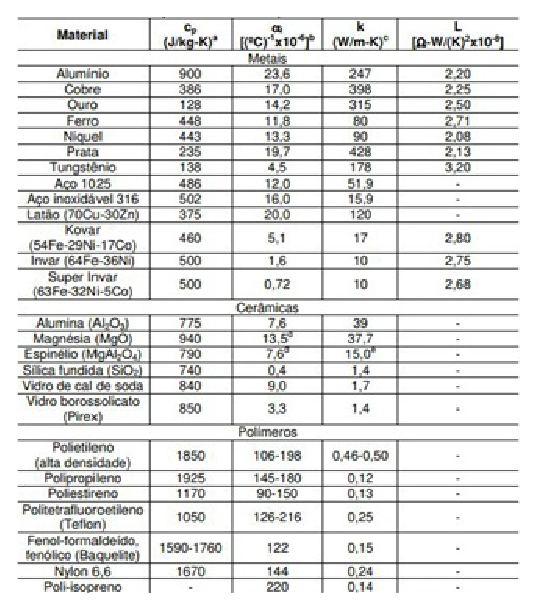
\includegraphics[scale=1]{figuras/Figura4tc.eps}
\end{table}
\\O comprimento total do tubo utilizado no sensor é de 6 m, com diâmetro interno de 4 mm e espessura 1mm, o valor da temperatura interna é de aproximadamente $50^0C$ e sua temperatura externa tem em torno de $30^0C$. A partir desses dados, e da equação ~\ref{eq3tc} conclui-se que o valor Q equivale a 464,89 W.
\section{Tubulações}
\subsection{Material}
Para as mangueiras e conectores da condução do líquido de arrefecimento, o material utilizado será o politetrafluoretileno (PTFE), popularmente conhecido como teflon. As principais características desse plástico fluorado é sua inércia química, estabilidade em altas e baixas temperaturas, excelentes propriedades elétricas e baixo coeficiente de atrito. 
As resinas de PTFE são opacas, cristalizadas e maleáveis. Quando aquecidas acima de 340ºC, tornam-se transparentes, amorfas e de tratamento relativamente difícil, sofrendo fraturas quando severamente deformadas. Ao serem resfriadas, voltam ao seu estado original. 
Geralmente são utilizadas em aplicações nas quais se aproveitam suas propriedades elétricas, químicas e mecânicas fora do comum, mas também em componentes de sistemas de transportes de fluidos, peças moldadas de ajuste e vedação, entre outros. 
A alta resistência ao calor e outras características do PTFE, listadas na tabela 02, foram os principais critérios utilizados para escolha desse material para a composição do projeto. 
\begin{table}[!htb]
	\centering
	\caption{Propriedades térmicas do PFTE}\label{tab2tc}
	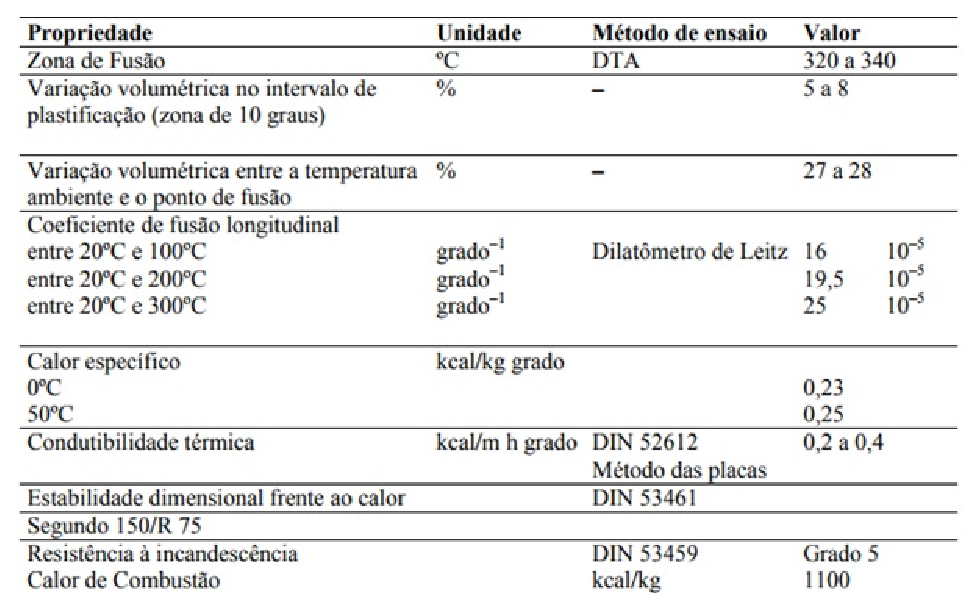
\includegraphics[scale=0.8]{figuras/Figura5tc.eps}
\end{table}
Já em relação ao adaptador que liga a pós-câmara ao sensor de pressão, será empregado o Aço Inoxidável (AISI 304L). A escolha do material foi determinada por meio das propriedades físicas e químicas, entre elas: o material apresenta boa resistência à corrosão e resistência à oxidação de até $850^oC$, permite excelente maquinabilidade, e é muito dúctil sendo de fácil estampagem e embutidura outras características são apresentadas na tabela~\ref{tab3tc}. 
\begin{table}[!htb]
	\centering
	\caption{Propriedades do AISI 304L}\label{tab3tc}
	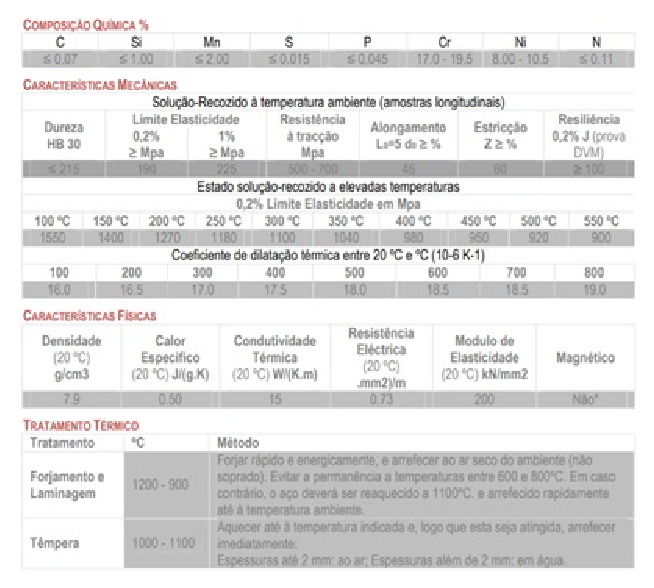
\includegraphics[scale=1]{figuras/Figura6tc.eps}
\end{table}
\newpage
\subsection{Dimensões}
De acordo com o modelo feito para o posicionamento da bomba, os materiais necessários, do sistema até a chegada ao sensor serão: 
\begin{itemize}
	\item \textbf{Comprimento da mangueira:} 6m;
	\item \textbf{Diâmetro da mangueira:} 4mm;
	\item \textbf{Numero de conexões em \emph{Cotovelo}:} 4 unidades;
	\item \textbf{Numero de conexões em \emph{Tê}:} 2 unidades;
\end{itemize}
Já para o tubo que conecta ao sensor é necessário um ducto de $diâmetro(Ø) =19mm$ por 100mm de comprimento. Dessa forma, conforme a imagem~\ref{fig7tc} abaixo, a qual refere-se ao corte horizontal do tubo percebe-se um furo com $diâmetro(Ø) =3mm$ na maior parte de extensão.
\begin{figure}[!htb]                  
	\centering                          
	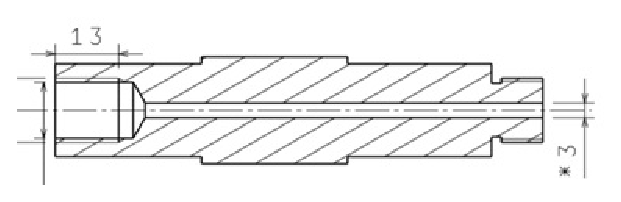
\includegraphics[scale=1]{figuras/Figura7tc.eps}
	\caption{Corte horizontal  do adaptador.} \label{fig7tc}              
\end{figure}
\newpage
Após a realização dos cálculos por meio de modelos matemáticos Newtonianos, é necessária a realização de simulações para que possam garantir que as operações foram efetuadas corretamente e assim, diminuir a porcentagem de erros e riscos.
Assim, foi então feita uma simulação por meio do Software ANSYS versão R18.1 Academic para determinar sua temperatura de ponta, assumindo-se o adaptador como um cilindro perfeito de diâmetro igual a 19mm e com comprimento de 100mm da mesma forma admitiu-se as propriedades dele em temperatura de 1000 ºC mais próximas encontradas na bibliografia que foram:
\begin{itemize}
	\item \textbf{Condutividade térmica:} 21.4 W/K.m;
	\item \textbf{temperatura ambiente:} $30^oC$;
	\item \textbf{Gradiente de condução:} 25 no sentido da seção;
\end{itemize}
A partir dessas aproximações foi gerado o seguinte gráfico no simulador ANSYS (figura~\ref{fig8tc}).
\begin{figure}[!htb]                  
	\centering                          
	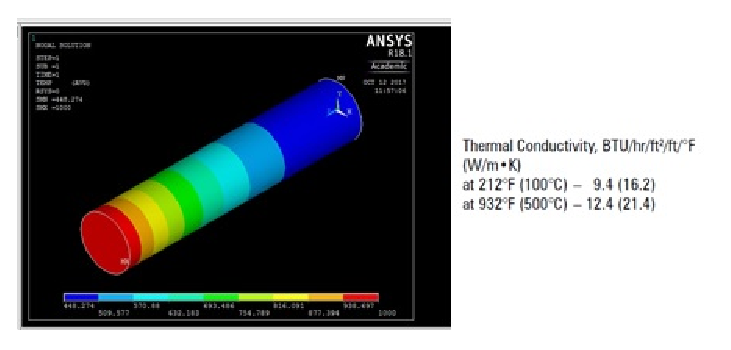
\includegraphics[scale=1]{figuras/Figura8tc.eps}
	\caption{Transmissão de calor no cilindro maciço .} \label{fig8tc}              
\end{figure}
\\Consequentemente, para uma segunda avaliação do conector o software utilizado foi o ANSYS versão R18.2 Academic. Assim, para realizar o estudo termodinâmico do tubo, o qual liga a pós-câmara ao sensor de pressão é empregado o Steady-State Thermal (Estado Térmico Estacionário), entretanto para uma maior precisão é necessária a realização de um estudo em um estado transiente, que depende do menor e maior tempo de execução do motor.
Posteriormente, o modo de simulação termodinâmica utilizado foi a convecção forçada de uma superfície para um fluido em movimento. Dessa forma abrange dois mecanismos de transferência de calor: o movimento molecular aleatório (difusão) e o movimento global do fluido.  
Com tal característica, utilizou-se  como geometria um cilindro de 19 mm de diâmetro com um furo no seu interior de 3mm de diâmetro, uma vez que a versão de software que foi utilizada não é compatível com o formato (\emph{CAD}) do Cátia realizado pelo grupo de estruturas.\\
Dessa forma, a partir da simulação apresentada conclui-se que não existem grandes alterações no resultado final comparando, a simulação de um cilindro sólido com uma simulação de um cilindro perfurado. Portanto, os cálculos realizados para cilindro são compatíveis com o adaptador e estão na faixa de tolerância de erros.\\
Na simulação aplica-se uma malha média (figura ~\ref{fig10tc}) e infere-se que a temperatura do exterior e do interior em um estado inicial sejam as mesmas de $30^oC$ (figura ~\ref{fig11tc}). Logo depois, utiliza uma temperatura que atinja uma máxima de $1000^oC$ linearmente, conforme os parâmetros da simulação apresentados anteriormente. Do mesmo modo, emprega a ferramenta de convecção na geometria que fica em contato com o fluido do interior da câmara do motor.
\begin{figure}[!htb]                  
	\centering                          
	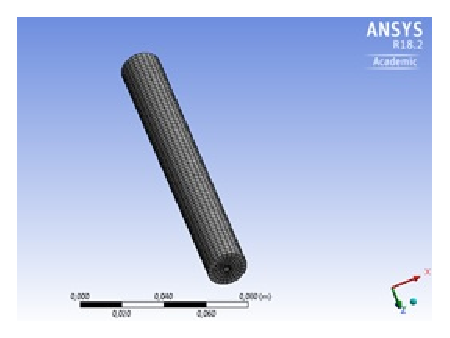
\includegraphics[scale=0.8]{figuras/Figura10tc.eps}
	\caption{Malha média inserida para realizar adição de temperaturas.} \label{fig10tc}              
\end{figure}
\begin{figure}[!htb]                  
	\centering                          
	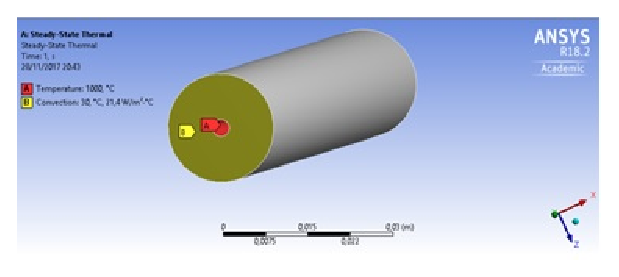
\includegraphics[scale=0.8]{figuras/Figura11tc.eps}
	\caption{Adaptador após as temperaturas inseridas.} \label{fig11tc}              
\end{figure}
\\Entretanto,  como o software utilizado foi uma versão de estudante obteve-se várias dificuldades, dentre elas: problemas com a especificação do material 304 L que  não era disponível na biblioteca geral “Engineering Data Sources”. Da mesma forma que, não tem compatibilidade com o cad realizado pelo grupo de estruturas e também por se tratar de uma simulação muito densa é necessário colocar uma malha média não tão precisa, uma vez que os computadores utilizados pelos alunos não suportam uma maior precisão. Outro fator limitante é usar duas temperaturas, uma temperatura ambiente na parte exterior e uma temperatura de $1000^oC$ que atinge a face inferior do cilindro, além de realizar um processo de convecção que sempre excedem os problemas numéricos e matemáticos do programa disponíveis para essa versão.\\ 
Apesar dessas dificuldades de simulação foi possível realizar uma simulação do adaptador com furo na parte mecânica do software ANSYS, considerando os mesmos padrões descritos anteriormente e seguindo alguns pontos de acordo com o comprimento do adaptador. Dessa forma foi possível analisar melhor a distribuição da temperatura no adaptador, obtendo a solução nodal seguinte: 
\begin{figure}[!htb]                  
	\centering                          
	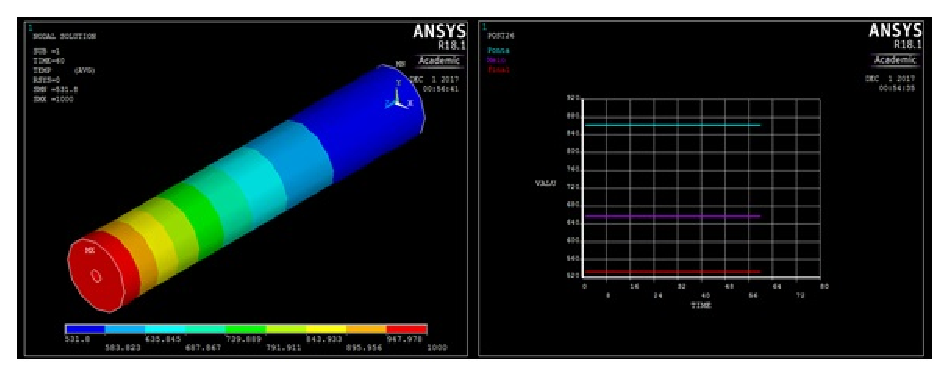
\includegraphics[scale=0.8]{figuras/Figura12tc.eps}
	\caption{Solução nodal e pontos específicos no comprimento} \label{fig12tc}              
\end{figure}
\section{Análise de Riscos}
Visto que o nosso grupo se dispõe apenas de ferramentas teóricas e simulações, seus riscos também se mantêm em tal perspectiva de forma que os únicos riscos existentes em tal processo sejam apenas técnicos e administrativos.
\subsection{Análise de Riscos Técnicos}
Nas utilizações das fórmulas e nas simulações podem existir erros contidos tanto na medição das variáveis iniciais, determinando assim uma propagação de erros muito grande levando em consideração o processo inteiro e a utilização de medidas experimentais industriais sem erro definido aumentando assim sua variabilidade. Pensando nisso, utilizando uma medida de contingência, a solução utilizada no projeto e aconselhada pelos professores é a simplificação e a utilização de fatores de seguranças mais razoáveis que a média, de forma que o custo benefício e solução do projeto sejam viáveis assim , todo e qualquer erro pode influenciar custo de produção baixo, não alterando significativamente o projeto. \\
A utilização de softwares também diminui consideravelmente o erro visto que sua capacidade para erros é menor de acordo com o grau da simulação. As únicas medidas de contenção que se restringe à essa parte é a reavaliação dos processos e sua imediata substituição pelos dados revisados. Sendo assim, uma vez observadas as falhas e soluções para tal, o grupo utilizou das informações coletadas para aprimorar o projeto a fim de reduzir o máximo suas possíveis limitações.
\subsection{Análise de Riscos Administrativos}
Os riscos mais prováveis em nossa desenvolvimento visto que nossa natureza estudantil nos leva a erros administrativos, a utilização de recursos humanos à sua potencialidade foi um dos problemas encontrados pelo grupo e o controle de pessoal, de forma que esses poderiam desestruturar o funcionamento, sendo eles o descumprimento de prazos, falta de pessoal, escopo incoerente, falta de priorização de tarefas  e impossibilidade de reuniões os maiores contribuintes nessa soma.
\section{Orçamentos}
\begin{table}[htbp]
	\centering
	\caption{Orçamento para equipe de transmissão de calor}
	\begin{tabular}{|c|c|}
		\toprule
		\rowcolor[rgb]{ .851,  .882,  .949} \multicolumn{1}{|c|}{\multirow{5}[2]{*}{\textbf{Mão de obra}}} & \multicolumn{1}{p{10.43em}|}{\cellcolor[rgb]{ 1,  1,  1}18 horas mensais para cada estudante} \\
		\rowcolor[rgb]{ .851,  .882,  .949}       & \multicolumn{1}{p{10.43em}|}{\cellcolor[rgb]{ 1,  1,  1} 5 estagiários } \\
		\rowcolor[rgb]{ .851,  .882,  .949}       & \multicolumn{1}{p{10.43em}|}{\cellcolor[rgb]{ 1,  1,  1}Usando um salário base de R\$1.000,00 de 120 horas mensais.} \\
		\rowcolor[rgb]{ .851,  .882,  .949}       & \cellcolor[rgb]{ 1,  1,  1} \\
		\rowcolor[rgb]{ .851,  .882,  .949}       & \multicolumn{1}{p{10.43em}|}{\cellcolor[rgb]{ 1,  1,  1}R\$ 150,00 * 5= R\$ 750,00 } \\
		\midrule
		\rowcolor[rgb]{ .851,  .882,  .949} \multicolumn{1}{|c|}{\multirow{2}[2]{*}{\textbf{Software Ansys}}} & \multicolumn{1}{p{10.43em}|}{\cellcolor[rgb]{ 1,  1,  1}Versão estudante com algumas limitações} \\
		\rowcolor[rgb]{ .851,  .882,  .949}       & \cellcolor[rgb]{ 1,  1,  1}R\$ 0,00 \\
		\bottomrule
	\end{tabular}
	\label{tabBtc}
\end{table}

\section{Resultados}
Primeiramente, o líquido escolhido foi a água pelas suas propriedades e pela facilidade encontrada para análises com base em dados disponibilizados pelo fabricante, assim como, auxilia na praticidade dos cálculos, além da facilidade de obtenção do material sendo gratuito e em grande quantidade. A escolha foi considerada com base em datasheets, contextualização do projeto para materiais de fácil aquisição e cálculos.\\
Consequentemente, as determinações dos principais parâmetros para o projeto foram formuladas a partir das análises teóricas e depois foram comprovadas pelo uso do simulador Ansys. De modo similar, as escolhas dos materiais são concretizadas pelas operações, adaptando as propriedades físicas e químicas de cada material aos requisitos térmicos do sistema.
Após todos esses passos, os resultados encontrados nas funções que cabiam ao grupo, após a simulação do cilindro, foi de 450ºC na ponta do adaptador, a temperatura da água não ultrapassa 60ºC e o sensor sobreviverá à temperatura que se encontra no motor se o sistema de arrefecimento funcionar corretamente, realizando as medições necessárias entre os períodos de tempo do teste, sendo eles entre 15 e 60 segundos.\\ Lembrando que as análises e simulações foram feitas de levando em consideração o “worst-case scenario”, isto é, quando o pior das situações acontece, nesse caso, com a maior temperatura possível e sem proteção térmica no sistema.\\
As transmissões encontradas foram baseadas sem levar em conta a proteção térmica, condução no cilindro e radiação no resfriamento pela diferença de temperatura, etc. Logo, Independentemente do sistema de proteção térmica, a previsão do fluxo de calor é uma tarefa de extrema importância, tanto em motores de foguete a propelente líquido quanto em motores a propelente sólido pois se trata de um aspecto que limita a performance do propulsor, forçando muitas vezes o processo de combustão ser ajustado para operar fora do ponto estequiométrico dos propelentes envolvidos para reduzir a temperatura dos gases quentes, evitando extrair a máxima eficiência energética dos propelentes (PATIRE JR, 2010). 

     
